%%
% This is an Overleaf template for presentations
% using the TUM Corporate Desing https://www.tum.de/cd
%
% For further details on how to use the template, take a look at our
% GitLab repository and browse through our test documents
% https://gitlab.lrz.de/latex4ei/tum-templates.
%
% The tumbeamer class is based on the beamer class.
% If you need further customization please consult the beamer class guide
% https://ctan.org/pkg/beamer.
% Additional class options are passed down to the base class.
%
% If you encounter any bugs or undesired behaviour, please raise an issue
% in our GitLab repository
% https://gitlab.lrz.de/latex4ei/tum-templates/issues
% and provide a description and minimal working example of your problem.
%%

\PassOptionsToClass{onlytextwidth}{beamer}

\documentclass[
  german,            % define the document language (english, german)
  aspectratio=169,    % define the aspect ratio (169, 43)
  % handout=2on1,       % create handout with multiple slides (2on1, 4on1)
  % partpage=false,     % insert page at beginning of parts (true, false)
  % sectionpage=true,   % insert page at beginning of sections (true, false)
]{tumbeamer}


% load additional packages
\usepackage{tikz}
\usepackage{circuitikz}
\usepackage{url}
\usepackage{hyperref}
\usepackage{pgf}
\usepackage{pgfplots}
\usepackage{babel}[ngerman]
\usepackage{csquotes}[autostyle]
\usepackage[useregional]{datetime2}
\usepackage{float}
\usepackage{graphicx}
\usepackage{amsmath}
\usepackage{xcolor}
\usepackage[cache=true]{minted}
\usemintedstyle{borland}
\usepackage{listings}
\usepackage{tikz-timing}


% tikz
\usetikzlibrary{overlay-beamer-styles}
\usetikzlibrary{arrows,backgrounds,positioning,shapes,patterns,patterns.meta,matrix,arrows,shapes.geometric}
\usetikzlibrary{matrix, fit}

% requires circuitikz >= 1.1.0
% for distros with older distributions, install TeX Live manually
% instead of using your package manager
% see: https://tug.org/texlive/quickinstall.html
\ctikzset{logic ports=european}

% minted
\setminted{
    fontsize=\small, 
    frame=none,
    breaklines=true,
}

% image path
\graphicspath{ {./resources/} }

% beamer
\setbeamercolor{footnote}{fg=black}
\setbeamercolor{footnote mark}{fg=black}

% presentation metadata
\title{Übung 08: Maschinensprache \\und Single-Cycle-Prozessor}
\subtitle{Einführung in die Rechnerarchitektur}
\author{Niklas Ladurner}

\institute{\theChairName\\\theDepartmentName\\\theUniversityName}
\date{\DTMdisplaydate{2024}{12}{06}{-1}}

\footline{\insertauthor~|~\insertshorttitle~|~\insertshortdate}


% macro to configure the style of the presentation
\TUMbeamersetup{
  title page = TUM tower,         % style of the title page
  part page = TUM toc,            % style of part pages
  section page = TUM toc,         % style of section pages
  content page = TUM more space,  % style of normal content pages
  tower scale = 1.0,              % scaling factor of TUM tower (if used)
  headline = TUM threeliner,      % which variation of headline to use
  footline = TUM default,         % which variation of footline to use
  % configure on which pages headlines and footlines should be printed
  headline on = {title page},
  footline on = {every page, title page=false},
}

\begin{document}

\maketitle

\begin{frame}[c]{Feedback}{}
	\begin{columns}[c]
		\begin{column}{0.5\textwidth}
			\begin{center}
				\LARGE  \href{https://t1p.de/era2425}{t1p.de/era2425}\\
				
\includegraphics[height=0.5\textheight]{feedback_qr.png}
			\end{center}
		\end{column}
		\begin{column}{0.5\textwidth}
			\begin{center}
				\LARGE  \href{https://home.in.tum.de/~ladu/}{home.in.tum.de/\string~ladu/}\\
				
\includegraphics[height=0.5\textheight]{website_qr.png}
			\end{center}
		\end{column}
	\end{columns}
\end{frame}

\begin{frame}[c, fragile]{}{}
	\begin{center}
		\LARGE  Keine Garantie für die Richtigkeit der Tutorfolien.

		\Large Bei Unklarheiten/Unstimmigkeiten haben VL/ZÜ-Folien recht!
	\end{center}
\end{frame}

\begin{frame}[c, fragile]{RISC-V Instruktionstypen}{}
	\begin{itemize}
		\item R-Typ: Register-Register-Operationen (bspw. \texttt{add}, \texttt{sub}, \texttt{sll})
		\item I-Typ: kleine Immediates (12 Bit) und Ladebefehle (bspw. \texttt{jalr}, \texttt{lw}, \texttt{ori})
		\item S-Typ: Speicherbefehle (bspw. \texttt{sw}, \texttt{sh})
		\item B-Typ: Branches (bedingte Sprünge) (bspw. \texttt{beq}, \texttt{blt}, \texttt{bgtu})
		\item U-Typ: große Immediates (20 Bit) (bspw. \texttt{lui}, \texttt{auipc})
		\item J-Typ: Jumps (unbedingte Sprüge) (\texttt{jal})
		\item R4-Typ: Floating-Point-Operationen, für ERA nicht relevant
	\end{itemize}
\end{frame}

\begin{frame}[c, fragile]{Assemblierung zu Maschinensprache}{}
	\begin{columns}[c]
		\begin{column}{0.5\textwidth}
			\begin{itemize}
				\item RV32: Instruktionsgröße von 32 Bit (compressed instructions 16 Bit)
				\item Übersetzung in CISC-Architekturen aufwendiger (vgl. IA-32: 2552 Seiten Instruction Reference)
				\item Instruktionen selben Typs werden haben gleiches Instruktionslayout
				\item alle benötigten Tabellen sind in der Klausur gegeben
			\end{itemize}
		\end{column}
		\begin{column}{0.5\textwidth}
			\begin{center}
				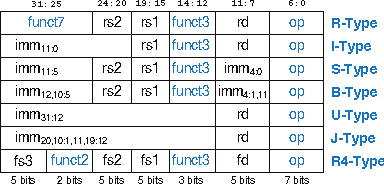
\includegraphics[width=\textwidth]{w08_risc_v_types.pdf}\\
			\end{center}
			\centering
			\tiny (Quelle: Vorlesungsmaterialien ERA)
		\end{column}
	\end{columns}
\end{frame}

\begin{frame}[c, fragile]{Assemblierung zu Maschinensprache: Beispiel}{}
	\begin{center}
		\large\texttt{xor t2, t1, t0}\\
		\scriptsize
		\begin{table}[]
			\begin{tabular}{|l|l|l|l|l|}
				\hline
				\rowcolor[HTML]{0078C3}
				{\color{white}\textbf{op}} & {\color{white}\textbf{funct3}} & {\color{white}\textbf{funct7}} & {\color{white}\textbf{Type}} & {\color{white}\textbf{Instruction}} \\ \hline
				0110011 (51)               & 100                            & 0000000                        & R                            & \texttt{xor rd, rs1, rs2}           \\ \hline
			\end{tabular}
		\end{table}

		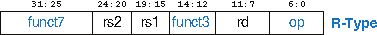
\includegraphics[width=0.59\textwidth]{w08_r_type.pdf}
	\end{center}

	\begin{enumerate}
		\item \texttt{xor} $\rightarrow$ R-Typ
		\item \texttt{t0} $\rightarrow$ \texttt{x5} (rs2), \texttt{t1} $\rightarrow$ \texttt{x6} (rs1), \texttt{t2} $\rightarrow$ \texttt{x7} (rd)
		\item funct7, funct3, op aus Tabelle ablesen
	\end{enumerate}
	\begin{center}
		\Large
		$(0000000\;00101\;00110\;100\;00111\;0110011)_2 = \textrm{0x005343B3}$
	\end{center}

\end{frame}



\begin{frame}[c]{RISC-V Single-Cycle-Prozessor}{}
	\begin{center}
		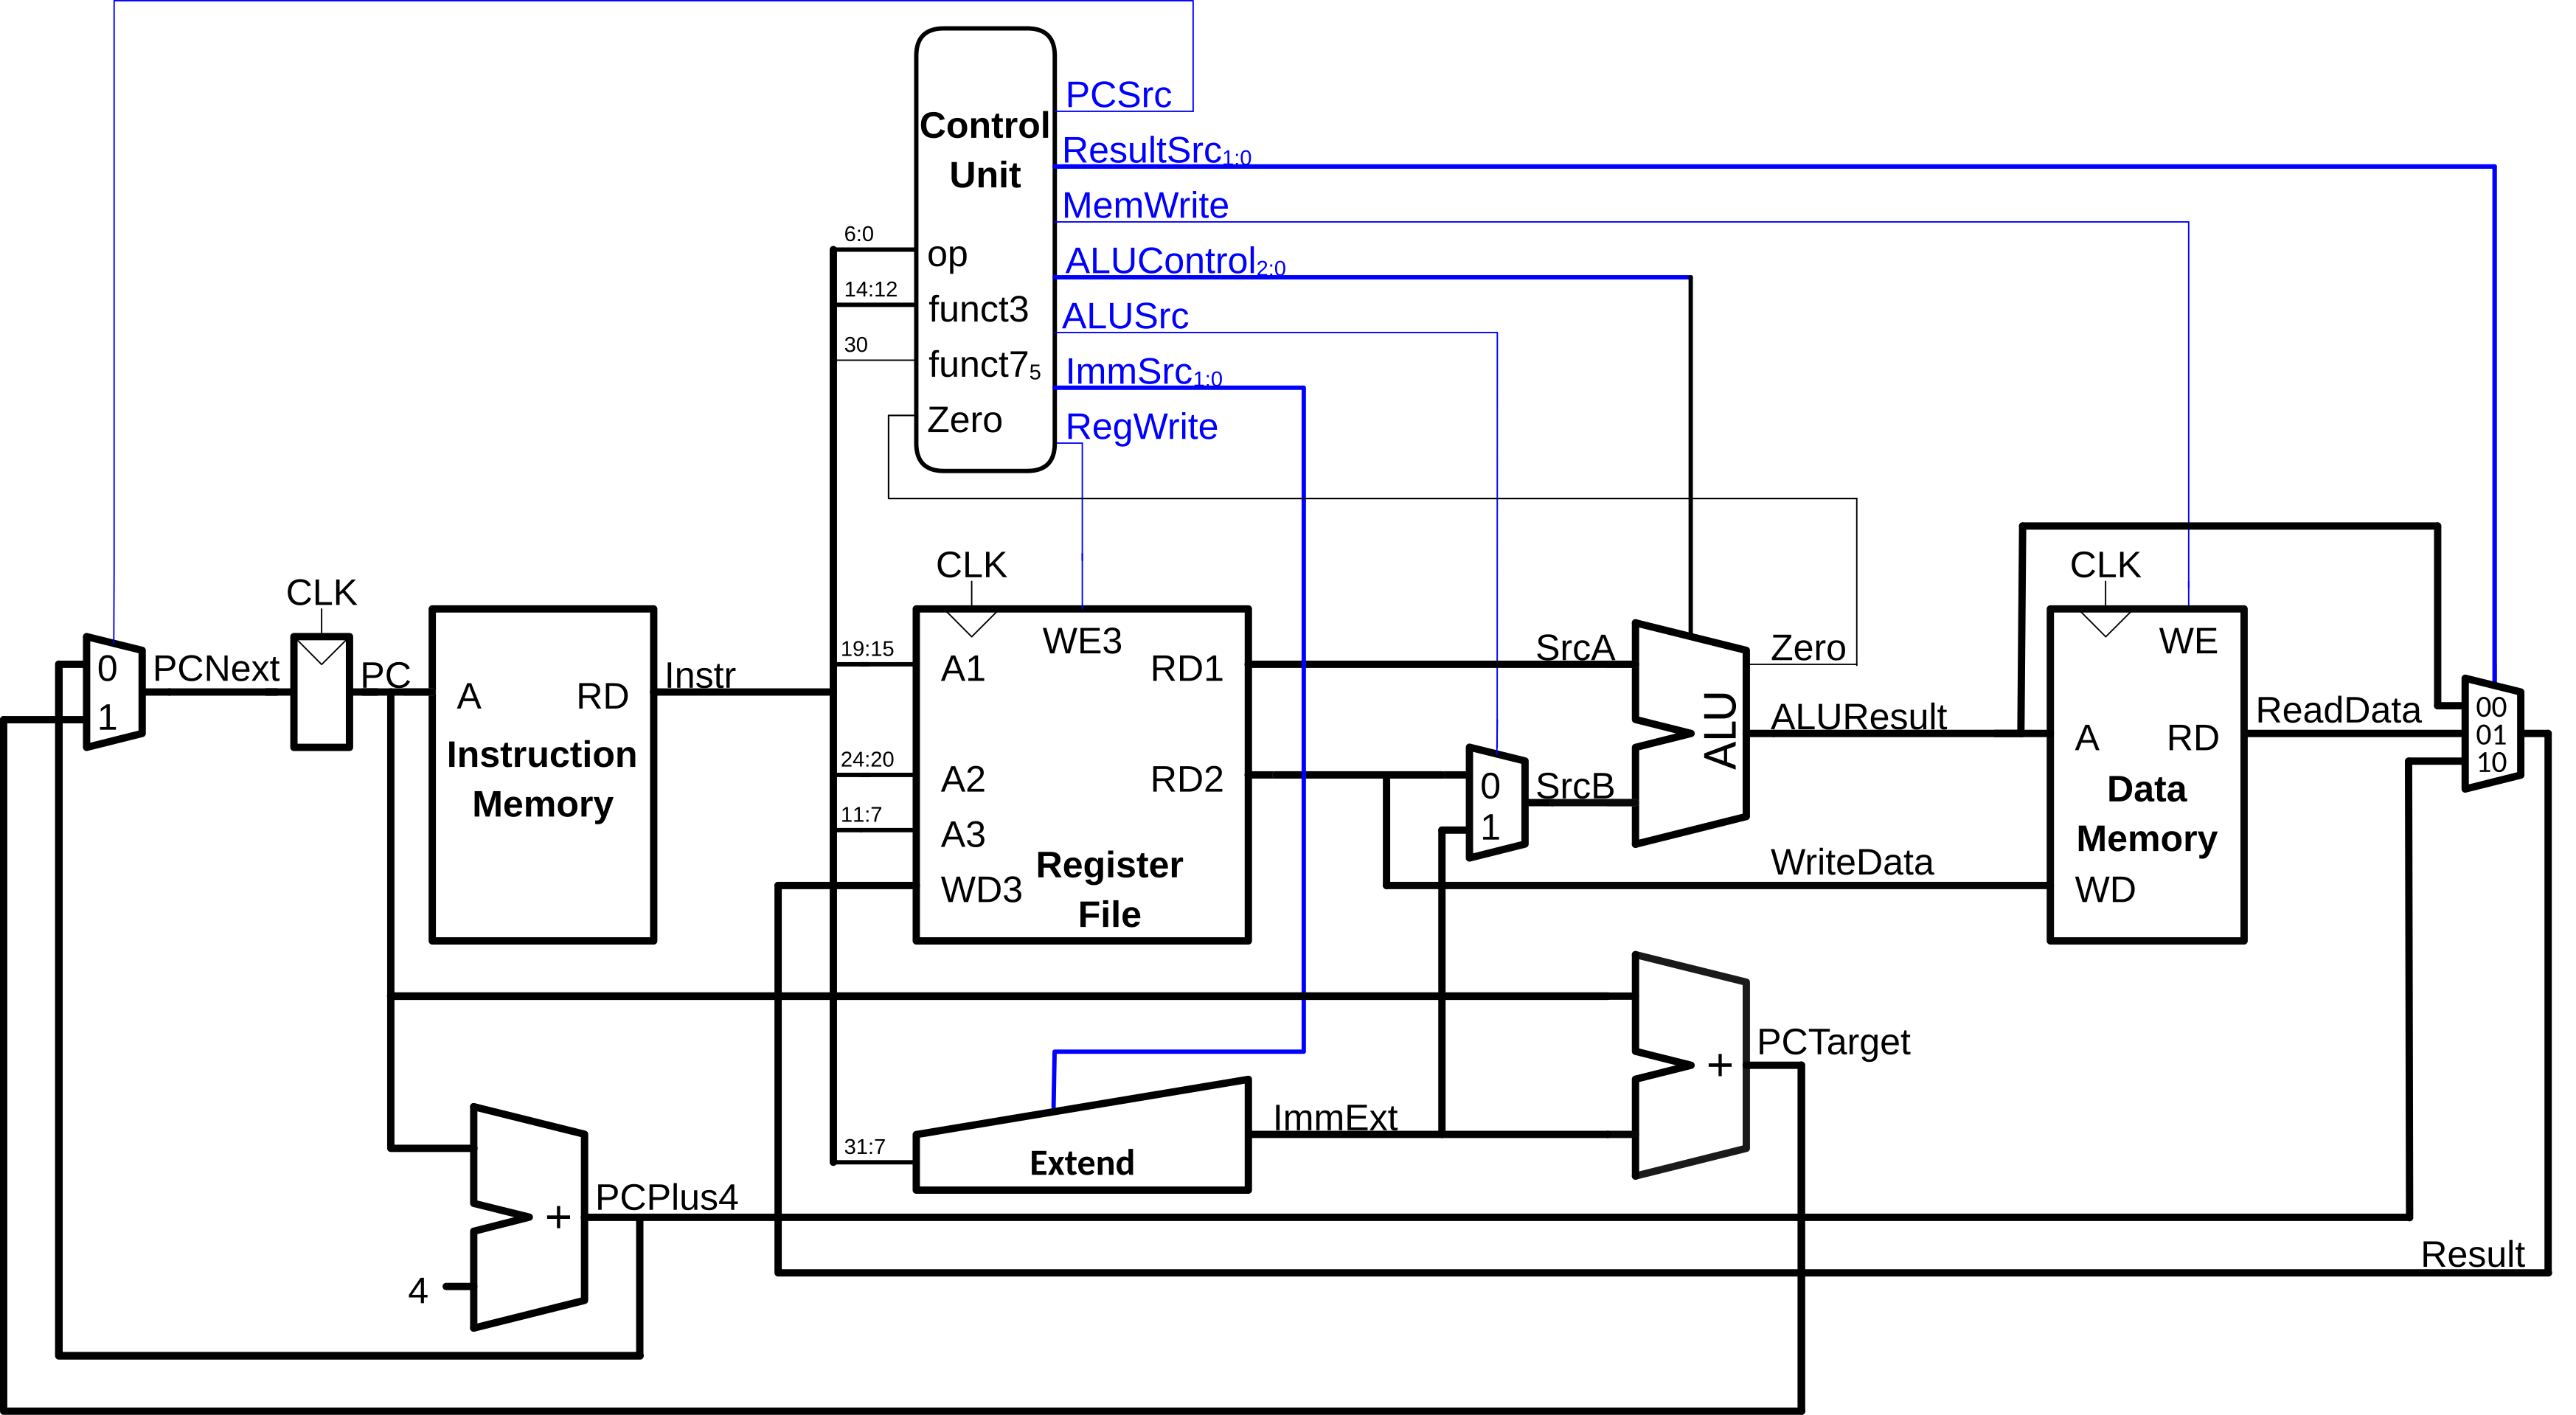
\includegraphics[width=0.8\textwidth]{w08_single_cycle.png}
	\end{center}
	\centering
	\tiny (Quelle: Vorlesungsmaterialien ERA)
\end{frame}

\begin{frame}[c, fragile]{}{}
	\begin{center}
		\LARGE Fragen?
	\end{center}
\end{frame}

\begin{frame}[c, fragile]{Artemis-Hausaufgaben}{}
	\begin{itemize}
		\item \enquote{H08 --- Single-Cycle-Prozessorerweiterung} bis 15.12.2024 23:59 Uhr
		\item Erweiterung des einfachen Single-Cycle-Prozessors
		\item {\ttfamily{xor}} (R-Typ) und {\ttfamily{jalr}} (I-Typ)
		\item Oft auch Prozessorerweiterung als Klausuraufgabe!
	\end{itemize}
\end{frame}

\begin{frame}[c, fragile]{Links}{}
	\begin{itemize}
		\item Zulip: \href{https://zulip.in.tum.de/#narrow/stream/2661-ERA-Tutorium---Do-1600-1}{\enquote{ERA Tutorium - Do-1600-1}}
		      bzw. \href{https://zulip.in.tum.de/#narrow/stream/2675-ERA-Tutorium---Fr-1500-2 }{\enquote{ERA Tutorium - Fr-1500-2}}
		\item \href{https://www.moodle.tum.de/course/view.php?id=100633}{ERA-Moodle-Kurs}
		\item \href{https://artemis.in.tum.de/courses/401}{ERA-Artemis-Kurs}
		\item \href{https://courses.edx.org/assets/courseware/v1/f06a2dc0c856f60ec0711e9f5e1c98cf/asset-v1:HarveyMuddX+ENGR85B+1T2023+type@asset+block/FinalReferences.pdf}{Prozessor-Assets (kein offizielles Material!)}
		\item \href{https://riscvasm.lucasteske.dev/}{RISC-V Assembler}
	\end{itemize}
\end{frame}

\maketitle

\end{document}
